\documentclass{extbook}[14pt]
\usepackage{multicol, enumerate, enumitem, hyperref, color, soul, setspace, parskip, fancyhdr, amssymb, amsthm, amsmath, latexsym, units, mathtools}
\everymath{\displaystyle}
\usepackage[headsep=0.5cm,headheight=0cm, left=1 in,right= 1 in,top= 1 in,bottom= 1 in]{geometry}
\usepackage{dashrule}  % Package to use the command below to create lines between items
\newcommand{\litem}[1]{\item #1

\rule{\textwidth}{0.4pt}}
\pagestyle{fancy}
\lhead{}
\chead{Answer Key for Module7 Version C}
\rhead{}
\lfoot{5507-6544}
\cfoot{}
\rfoot{test}
\begin{document}
\textbf{This key should allow you to understand why you choose the option you did (beyond just getting a question right or wrong). \href{https://xronos.clas.ufl.edu/mac1105spring2020/courseDescriptionAndMisc/Exams/LearningFromResults}{More instructions on how to use this key can be found here}.}

\textbf{If you have a suggestion to make the keys better, \href{https://forms.gle/CZkbZmPbC9XALEE88}{please fill out the short survey here}.}

\textit{Note: This key is auto-generated and may contain issues and/or errors. The keys are reviewed after each exam to ensure grading is done accurately. If there are issues (like duplicate options), they are noted in the offline gradebook. The keys are a work-in-progress to give students as many resources to improve as possible.}

\rule{\textwidth}{0.4pt}

\begin{enumerate}\litem{
Solve the rational equation below.
\[ \frac{7x}{3x + 7} + \frac{-6x^{2}}{15x^{2} +44 x + 21} = \frac{-6}{5x + 3} \]The solution is \( \text{All solutions are invalid or lead to complex values in the equation.} \).\begin{enumerate}[label=\Alph*.]
\textbf{Plausible alternative answers include:}* The equation leads to solving $41x^{2} +39 x + 42=0$, which leads to complex solutions. This is the correct option.
$x = -2.333$, which corresponds to solving $3x + 7 = 0$ and treating it as a solution to the equation.
$x = -2.333 \text{ and } x = -0.600$, which corresponds to solving $3x + 7 = 0$ and $5x + 3 = 0$ and treating them as solutions to the equation.
$x = -0.600$, which corresponds to solving $5x + 3 = 0$ and treating it as a solution to the equation.
$x = -1.369 \text{ and } x = 0.418$, which corresponds to making the discriminant from the Quadratic Formula positive to avoid complex solutions.
\end{enumerate}

\textbf{General Comment:} Distractors are different based on the number of solutions. Remember that after solving, we need to make sure our solution does not make the original equation divide by zero!
}
\litem{
Determine the domain of the function below.
\[ f(x) = \frac{6}{15x^{2} +43 x + 30} \]The solution is \( \text{All Real numbers except } x = -1.667 \text{ and } x = -1.200. \).\begin{enumerate}[label=\Alph*.]
\textbf{Plausible alternative answers include:}This corresponds to thinking the denominator has complex roots or that rational functions have a domain of all Real numbers.
All Real numbers except $x = -1.667$, which corresponds to removing only 1 value from the denominator.
All Real numbers except $x = -30.000$ and $x = -15.000$, which corresponds to not factoring the denominator correctly.
All Real numbers except $x = -1.667$ and $x = -1.200$, which is the correct option.
All Real numbers except $x = -30.000$, which corresponds to removing a distractor value from the denominator.
\end{enumerate}

\textbf{General Comment:} Recall that dividing by zero is not a real number. Therefore the domain is all real numbers \textbf{except} those that make the denominator 0.
}
\litem{
Solve the rational equation below.
\[ \frac{63}{-56x + 28} + 1 = \frac{63}{-56x + 28} \]The solution is \( \text{all solutions are invalid or lead to complex values in the equation.} \).\begin{enumerate}[label=\Alph*.]
\textbf{Plausible alternative answers include:}$x = 0.500 \text{ and } x = 0.500$, which corresponds to getting the correct solution and believing there should be a second solution to the equation.
$x = 0.500$, which corresponds to not checking if this value leads to dividing by 0 in the original equation and thus is not a valid solution.
$x = -0.500 \text{ and } x = 0.500$, which corresponds to getting the correct solution and believing there should be a second solution to the equation.
*$x = 0.500$ leads to dividing by 0 in the original equation and thus is not a valid solution, which is the correct option.
$x = -0.500$, which corresponds to not distributing the factor $-56x + 28$ correctly when trying to eliminate the fraction.
\end{enumerate}

\textbf{General Comment:} Distractors are different based on the number of solutions. Remember that after solving, we need to make sure our solution does not make the original equation divide by zero!
}
\litem{
Solve the rational equation below.
\[ \frac{2}{-6x + 9} + 3 = \frac{4}{18x -27} \]The solution is \( x = 1.685 \).\begin{enumerate}[label=\Alph*.]
\textbf{Plausible alternative answers include:}This corresponds to thinking $x = 1.685$ leads to dividing by zero in the original equation, which it does not.
$x = -1.315$, which corresponds to not distributing the factor $-6x + 9$ correctly when trying to eliminate the fraction.
$x = -1.315 \text{ and } x = 1.685$, which corresponds to getting the correct solution and believing there should be a second solution to the equation.
* $x = 1.685$, which is the correct option.
$x = 1.389 \text{ and } x = 1.685$, which corresponds to getting the correct solution and believing there should be a second solution to the equation.
\end{enumerate}

\textbf{General Comment:} Distractors are different based on the number of solutions. Remember that after solving, we need to make sure our solution does not make the original equation divide by zero!
}
\litem{
Write an equation that can represent the function graphed below.

\begin{center}
    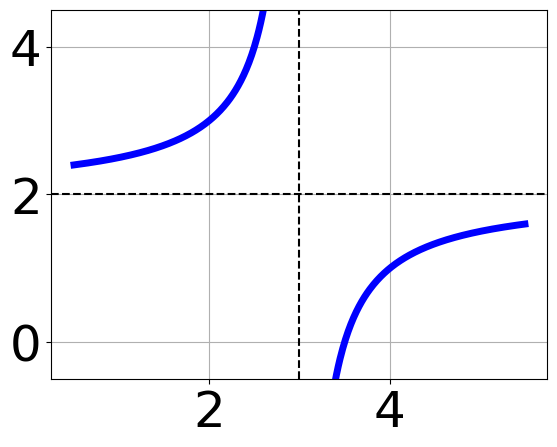
\includegraphics[width=0.5\textwidth]{../Figures/rationalGraphToEquationC.png}
\end{center}


The solution is \( f(x) = \frac{-1}{x - 3} + 2 \).\begin{enumerate}[label=\Alph*.]
\textbf{Plausible alternative answers include:}Corresponds to thinking the graph was a shifted version of $\frac{1}{x^2}$.
This is the correct option.
Corresponds to thinking the graph was a shifted version of $\frac{1}{x^2}$, using the general form $f(x) = \frac{a}{x+h}+k$, and the opposite leading coefficient.
Corresponds to using the general form $f(x) = \frac{a}{x+h}+k$ and the opposite leading coefficient.
This corresponds to believing the vertex of the graph was not correct.
\end{enumerate}

\textbf{General Comment:} Remember that the general form of a basic rational equation is $ f(x) = \frac{a}{(x-h)^n} + k$, where $a$ is the leading coefficient (and in this case, we assume is either $1$ or $-1$), $n$ is the degree (in this case, either $1$ or $2$), and $(h, k)$ is the intersection of the asymptotes.
}
\litem{
Sketch a graph that represents the equation below.
\[ f(x) = \frac{1}{(x - 1)^2} - 3 \]The solution is the graph below.
    \begin{center}
        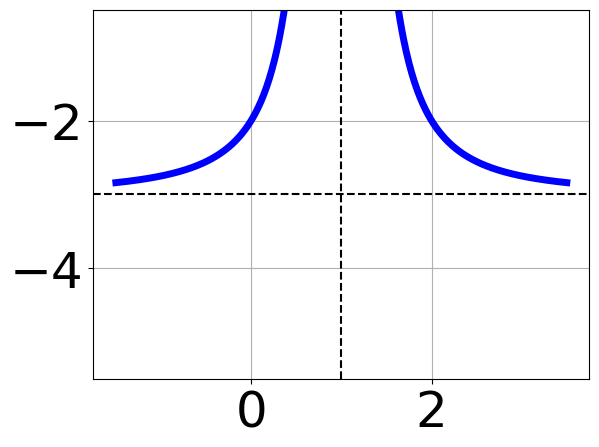
\includegraphics[width=0.3\textwidth]{../Figures/rationalEquationToGraphCC.png}
    \end{center}

\textbf{General Comment:} Remember that the general form of a basic rational equation is $ f(x) = \frac{a}{(x-h)^n} + k$, where $a$ is the leading coefficient (and in this case, we assume is either $1$ or $-1$), $n$ is the degree (in this case, either $1$ or $2$), and $(h, k)$ is the intersection of the asymptotes.
}
\litem{
Determine the domain of the function below.
\[ f(x) = \frac{3}{20x^{2} +3 x -9} \]The solution is \( \text{All Real numbers except } x = -0.750 \text{ and } x = 0.600. \).\begin{enumerate}[label=\Alph*.]
\textbf{Plausible alternative answers include:}All Real numbers except $x = -0.750$, which corresponds to removing only 1 value from the denominator.
All Real numbers except $x = -12.000$, which corresponds to removing a distractor value from the denominator.
This corresponds to thinking the denominator has complex roots or that rational functions have a domain of all Real numbers.
All Real numbers except $x = -0.750$ and $x = 0.600$, which is the correct option.
All Real numbers except $x = -12.000$ and $x = 15.000$, which corresponds to not factoring the denominator correctly.
\end{enumerate}

\textbf{General Comment:} Recall that dividing by zero is not a real number. Therefore the domain is all real numbers \textbf{except} those that make the denominator 0.
}
\litem{
Solve the rational equation below.
\[ \frac{-5x}{-3x -5} + \frac{-4x^{2}}{-9x^{2} -24 x -15} = \frac{5}{3x + 3} \]The solution is \( \text{There are two solutions: } x = -1.147 \text{ and } x = 1.147 \).\begin{enumerate}[label=\Alph*.]
\textbf{Plausible alternative answers include:}

* $x = -1.147 \text{ and } x = 1.147$, which is the correct option.


\end{enumerate}

\textbf{General Comment:} Distractors are different based on the number of solutions. Remember that after solving, we need to make sure our solution does not make the original equation divide by zero!
}
\litem{
Write an equation that can represent the function graphed below.

\begin{center}
    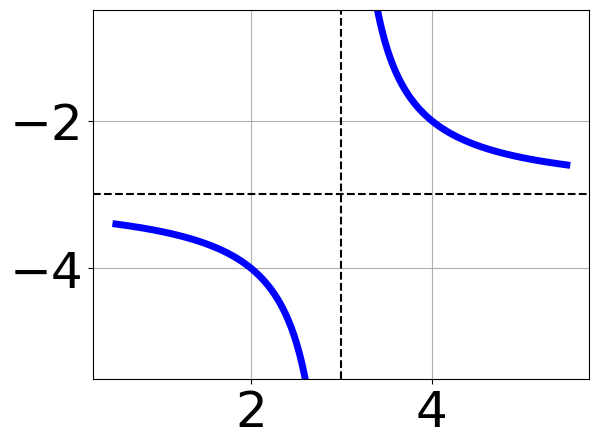
\includegraphics[width=0.5\textwidth]{../Figures/rationalGraphToEquationCopyC.png}
\end{center}


The solution is \( \text{None of the above as it should be } f(x) = \frac{1}{x - 3} - 3 \).\begin{enumerate}[label=\Alph*.]
\textbf{Plausible alternative answers include:}Corresponds to using the general form $f(x) = \frac{a}{x-h}+k$ and the opposite leading coefficient.
The $x$-value of the equation does not match the graph.
Corresponds to thinking the graph was a shifted version of $\frac{1}{x^2}$, using the general form $f(x) = \frac{a}{x-h}+k$, and the opposite leading coefficient.
Corresponds to thinking the graph was a shifted version of $\frac{1}{x^2}$.
None of the equation options were the correct equation.
\end{enumerate}

\textbf{General Comment:} Remember that the general form of a basic rational equation is $ f(x) = \frac{a}{(x-h)^n} + k$, where $a$ is the leading coefficient (and in this case, we assume is either $1$ or $-1$), $n$ is the degree (in this case, either $1$ or $2$), and $(h, k)$ is the intersection of the asymptotes.
}
\litem{
Sketch a graph that represents the equation below.
\[ f(x) = \frac{-1}{x - 3} - 3 \]The solution is the graph below.
    \begin{center}
        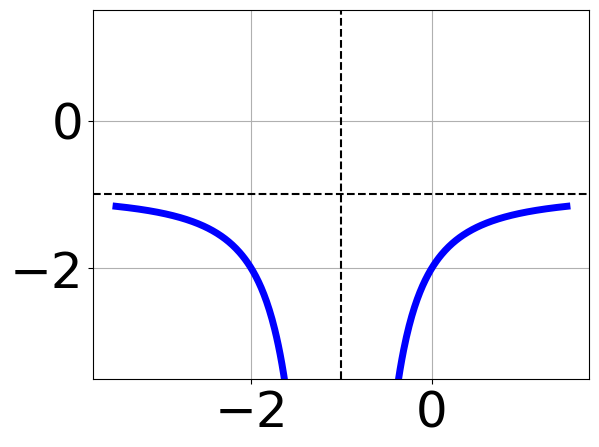
\includegraphics[width=0.3\textwidth]{../Figures/rationalEquationToGraphCopyAC.png}
    \end{center}

\textbf{General Comment:} Remember that the general form of a basic rational equation is $ f(x) = \frac{a}{(x-h)^n} + k$, where $a$ is the leading coefficient (and in this case, we assume is either $1$ or $-1$), $n$ is the degree (in this case, either $1$ or $2$), and $(h, k)$ is the intersection of the asymptotes.
}
\end{enumerate}

\end{document}